% !TeX program = xelatex
\documentclass[bachelor,english,draft,pdfdoc]{kentech-ucs}

\usepackage{amsmath,amssymb,booktabs,tabularx}
\usepackage{tikz}
\usetikzlibrary{arrows.meta,positioning}

\ifXeTeX
  \IfFontExistsTF{Noto Serif CJK KR}{\setmainhangulfont[AutoFakeSlant]{Noto Serif CJK KR}}{%
    \IfFontExistsTF{UnBatang}{\setmainhangulfont{UnBatang}}{%
      \IfFontExistsTF{NanumMyeongjo}{\setmainhangulfont{NanumMyeongjo}}{}}}
\fi

\title[eng-full]{Predicting the Next Attacker Action from Windows Audit Logs}
\title[kor]{윈도우 감사 로그를 이용한 공격자의 다음 행동 예측}
\department{BA}
\hypersetup{pdftitle={Predicting the Next Attacker Action from Windows Audit Logs}}

% In final mode, supply the author, advisor, examiners, and approval dates
% through the metadata commands in the KENTECH template.
\begin{document}
\begin{abstract}
PROPHET predicts which of 18 attacker actions comes next from the
Windows audit records received before a prediction cutoff. Under benign
workloads absent from every labeled training run, models sharing data
and architecture diverge across seeds, and the final training-batch
loss did not rank the seeds. Consensus distillation (CD), a standard
ensemble-distillation setup, trains one student toward the averaged
probabilities of five baseline models on unlabeled inputs from the new
workload. In a sealed in-house evaluation on new runs, mean negative
log-likelihood (NLL) fell from 0.0731 to 0.0276. On the public ADS-24
dataset, in a development comparison on inspected runs, the seed
standard deviation fell from 0.163 to 0.025, yet every distilled seed
of our model stayed worse than a training-prior baseline (NLL 1.830).
Three general encoders moved the same way in development comparisons,
though not every seed improved. CD narrowed the spread among these
checkpoints without removing the loss under environment shift.
% 근거: RECORD:166, 170 (v3, A+C FLAT); RECORD:218--219, 221, 234 (ADS-24);
% RECORD:294 (세 인코더). 세 인코더 결과는 자체·ADS-24 모두 이미 열람한 실행의
% 개발 비교다(answers 2026-11-24 07:10, 4번). "20 to 30 of 30"은 seed별 원자료를
% atlas에서 찾지 못해 뺐다. "not every seed improved"는 9장의 검증된 사례(ADS-24
% LSTM 기준 seed 2개가 기준선 아래, 학생은 0개)가 받친다. "training-prior baseline" = FIT 실행 동등 전술 빈도 예측기(8장 정의).
\end{abstract}

\begin{Engkeyword}
Next attacker action prediction, Underspecification, Seed instability,
Consensus distillation, Unlabeled adaptation, Windows audit logs
\end{Engkeyword}

\begin{korabstract}
본 연구는 예측 시점 전에 수신된 윈도우 감사 로그만으로 공격자가 다음에
수행할 행동을 18개 범주 중에서 예측한다. 정답이 붙은 학습 실행에 없던 정상
작업 조건에서는 같은 자료와 구조로 학습한 모델도 시드마다 성능이 크게
갈리며, 학습 마지막 미니배치의 손실로는 시드의 순위를 가릴 수 없었다. 이
흔들림을 줄이기 위해 기존의 앙상블 증류 방식을 적용하여, 새 작업 조건의
정답 없는 입력에서 기준 모델 다섯 개가 합의한 확률을 학생 모델이 따라
배우도록 한다. 학생은 기준 모델과 구조가 같아 추론 때도 단일 모델이다.
사전에 봉인한 자체 실험실 평가의 새 실행에서 평균 음의 로그우도는
0.0731에서 0.0276으로 낮아졌다. 공개 자료 ADS-24에서는 이미 열람한 평가
실행에서의 개발 비교로 시드 간 표준편차가 0.163에서 0.025로 줄었다. 세 가지
일반 인코더도 개발 비교에서 같은 방향을 보였다. 다만 모든 시드가 좋아지지는
않았고, ADS-24에서 우리 모델의 증류 시드는 모두 학습 자료의 전술 빈도만 쓰는
기준선(1.830)보다 손실이 높았다. 이 방법은 학습한 시드들 사이의 흔들림을 줄이지만, 환경 이동에 따른
성능 저하 자체를 없애지는 못한다.
\end{korabstract}

\begin{Korkeyword}
공격 행동 예측, 과소명세, 시드 불안정성, 합의 증류, 무라벨 적응, 윈도우 감사 로그
\end{Korkeyword}

\makecontents

\chapter{Introduction}
\label{ch:introduction}

During a multi-stage incident, an analyst may need to decide which
activity to investigate before the next attacker action is visible. A
forecast can prioritize this investigation by assigning probabilities
to plausible follow-up actions. It is important that the forecast
reflect the evidence that could actually have reached the analyst or
detector. Audit records carry an occurrence time, while their availability
to a predictor depends on when the collector receives them.

Consider a sequence of file-related activities involving two targets.
A termination record for one process may arrive after another process
starts. Benign activity on the host may add further start and termination
records in between. A model that treats the most recent exit code as the
result relevant to every subsequent decision can confuse the two
targets. A model that reconstructs a past prefix using all audit
records by occurrence time can also inadvertently give the predictor
information that the collector had yet to receive.

This thesis studies \textbf{next actual attacker action prediction}
from Windows audit logs. The label is the semantic category of the
first source-designated attacker action that actually starts after
the prediction boundary. The output is a distribution over 18 action
categories. An execution can provide several prediction rows, each
with its own evidence prefix and label. The task is evaluated at known
decision boundaries in a controlled environment. Inferring those
boundaries in an operational deployment is a separate problem.

PROPHET represents the evidence at each boundary in two complementary
forms. A gated recurrent unit summarizes the events in receipt order.
A target adapter connects observed events through process identity and
observed target membership. These links allow the predictor to use
the result of an operation on the relevant target even when unrelated
events intervene. A target-free path produces a prediction when the
observed prefix supplies no usable target relation.

The main question is whether linking events to the correct target
improves the forecast. On 64 new runs of previously evaluated
configurations, relation attention reduced execution-weighted negative
log likelihood (NLL) from 0.2171 to 0.0458 compared with a sequence-only
GRU. In a separate comparison, the target history model used the same
events and the same group sizes while event membership was exchanged.
On 127 previously examined executions, this exchange increased NLL
from 0.0584 to 0.0869. The first result measures the gain of the
target-aware predictor as a whole. The second tests whether correct
membership contributes to that gain in the target history model.

Chapter~\ref{ch:related} places these comparisons in the context of ATT\&CK, attack graphs, and prior forecasting systems.

The thesis defines an evaluation in which every forecast uses records
already received at its decision boundary. It tests observed target
membership against sequence and grouping controls, including new
executions with unfamiliar target names. It then tests how to present
recurrent history to the readout when benign activity is interleaved.
Chapter~\ref{ch:task} follows a recorded prediction to show what
the target links carry. Chapter~\ref{ch:method} defines the models,
and Chapters~\ref{ch:evaluation} and~\ref{ch:results} report the
comparisons and the conditions under which the gains hold.

\chapter{Background and Related Work}
\label{ch:related}
% 개요 2장. 옛 비교(EVENT GRU, 소속 교환, history placement) 설명과
% 옛 2.4절 "Evidence granularity and forecasting baselines"(빈도 기준선)는
% 부록 B(app:secondary-results)로 옮긴다. 옮기는 작업은 부록 B를 쓸 때 한다.
% 옛 원고의 sec:recorded-case, sec:membership 참조는 이 장에서 뺐다.

\section{ATT\&CK, the kill chain, and Attack Flow}
\label{sec:related-attack}

MITRE ATT\&CK organizes observed adversary behavior into tactics, the
objectives an activity serves, and techniques and sub-techniques, the
ways an objective is pursued~\cite{mitreintro}; the Windows matrix lists
the techniques that apply to that platform~\cite{mitrewindows}. We use
this vocabulary to situate the behaviors in our data, but the 18
prediction labels (Appendix~\ref{app:actions}) are finer than ATT\&CK
techniques. They name operations at the level of the controlled
procedures. A system information enumeration and a registry query are
both discovery activity, and they relate to System Information Discovery
and Query Registry respectively; merging them into one output would erase
exactly the distinction the classifier is asked to make. Conversely,
different command lines that implement the same operation share a label.
The label is the operation designated by the procedure and verified
against the actual process start, not an ATT\&CK identifier.

The intrusion kill chain of Hutchins et al.\ groups a campaign into
phases so that defenders can reason about where to interrupt
it~\cite{hutchins2011killchain}. At a single host decision, however,
several operations fall under the same phase, and knowing that an actor
is in discovery does not say which resource it will examine next. Attack
Flow goes further and represents the order of and dependencies between
adversary actions, so a flow can document a known incident or a
hypothetical scenario~\cite{mitreattackflow}. Both are descriptions
written with the whole sequence in view. A forecaster has only the prefix
received before the next action, and it must commit to a distribution
over that action before it is observed.

\section{Attack graphs and attack progression}
\label{sec:related-graphs}

Classical attack graphs model how conditions and exploits combine to
reach a security-relevant state. Sheyner et al.\ generate such graphs
automatically from a system model~\cite{sheyner2002graphs}, and MulVAL
derives security consequences from configuration facts with logic
rules~\cite{ou2005mulval}. An edge in these graphs is a relation
defined by the security model, which lets an analyst compare alternative
routes and find the conditions several routes depend on. What the graph
covers is bounded by the supplied facts and rules.

These graphs answer the question of which paths are possible under a
known configuration. PROPHET asks a different one: given the part of an
execution that has become visible, how probable is each concrete next
action? A feasible path is informative for the first question even if
it never occurs, while the second requires probabilities that can be
scored against what the actor actually did; several feasible responses
to the same preceding action carry no information about which one this
actor will take. B\u{a}b\u{a}lau et al.\ move attack graphs toward the second
question by building them from intrusion-detection alerts and using
them to forecast attacker actions~\cite{babalau2024forecasting}.

\section{Forecasting attacker actions and security events}
\label{sec:related-forecasting}

Learned forecasters work from observed event streams rather than from a
configuration model. Tiresias trains a recurrent model on histories of
security events from intrusion-prevention telemetry and predicts the
next event~\cite{shen2018tiresias}. DeepCASE builds a context for each
security event from the events preceding it and uses attention over
that context to group events for analyst triage~\cite{vanede2022deepcase}.
In both, inputs and outputs are events at the granularity of the
monitored stream. Our outputs are instead semantic attacker actions at a
known boundary, and the records arriving before that action can include
the termination of a previous operation and unrelated benign work.

A second group forecasts at the level of techniques or graphs.
CL-AP$^{2}$ builds a time-aware attack knowledge graph, portrays past
behavior by tactic, and estimates a trajectory from which it derives the
adversary's next technique~\cite{liu2024clap2}. EFI extracts attack-scene
graphs from threat intelligence reports, matches them against endpoint
provenance, and forecasts the next interactions with a technique-level
interpretation~\cite{zhu2024efi}. BiTA combines bidirectional GRU
aggregation with a Transformer in a temporal graph network to predict
future network alerts~\cite{nayeri2026bita}. Their outputs are a
technique, an interaction graph, or an alert, whereas ours is a single
normalized distribution over 18 action categories.

Provenance-based detectors share the host-level evidence but not the
forecasting goal. KAIROS detects intrusions in whole-system provenance
graphs and reconstructs the activity relevant to an
investigation~\cite{cheng2024kairos}, and ORTHRUS detects and attributes
attacks at the level of provenance nodes~\cite{jiang2025orthrus}. Their
outputs concern behavior that has already been observed. Chapter~\ref{ch:generality}
runs adaptations of ORTHRUS, BiTA, and CL-AP$^{2}$ on our inputs as a
reference point only; EFI is not adapted. In the versions of the
systems in this section that we consulted, we did not find results
reported across random seeds or under benign workloads absent from
training. This statement is limited to those versions and is not a
claim that such evaluations do not exist elsewhere.
% 근거: RECORD:477, 480. 각 원문 판본에서 seed 변동 보고 여부를 사람이
% 다시 확인해 주세요(표 tab:related-tasks 마지막 열과 같은 범위).

\section{Sequence models for logs}
\label{sec:related-sequence}

Our inputs are Windows process creation and termination records, Security
events 4688 and 4689~\cite{ms4688, ms4689}, read only as they become
available at the receipt boundary defined in Chapter~\ref{ch:task}
(Figure~\ref{fig:cutoff}). Sequence models for system logs are the
closest general architectures for such input. DeepLog trains an LSTM
\cite{hochreiter1997long} on sequences of normal log keys and flags an entry as
anomalous when it falls outside the predicted next
keys~\cite{du2017deeplog}. LogBERT replaces the recurrent model with a
Transformer encoder~\cite{vaswani2017attention} trained by self-supervised
objectives on log sequences~\cite{guo2021logbert}. The gated recurrent unit
(GRU)~\cite{cho2014gru} is the simpler recurrent cell that our baseline
predictor uses at the event level (Chapter~\ref{ch:method}).

Chapter~\ref{ch:generality} uses three encoders drawn from this
family: an LSTM encoder (DeepLog-style), a Transformer encoder
(LogBERT-style), and a plain GRU. These are adaptations of the encoders
to our supervised next-action task, not reproductions of DeepLog or
LogBERT. They do not use the anomaly-detection objectives or
pretraining of the original systems; LogitNorm, input-gradient
regularization, and the relational residual of our baseline are
removed; and their settings were chosen by validation inside the FIT
set only.
% 근거: RECORD:281, 478.

\section{Underspecification and model agreement}
\label{sec:related-underspec}

D'Amour et al.\ describe underspecification: a training pipeline can
return many predictors with equivalent held-in performance that behave
differently under deployment conditions, and the pipeline does not
choose among them~\cite{damour2020underspecification}. Their work
establishes and documents the phenomenon across domains. We measure it
on next attacker action prediction and then try to reduce it. Baek et
al.\ observe that, across models, agreement on in-distribution data and
agreement on shifted data are linearly related in the same way as
accuracy, which allows performance under shift to be estimated from
unlabeled data~\cite{baek2022agreement}. That line of work uses agreement to
estimate performance; we use agreement as a training signal, letting a
student follow the consensus of several models on unlabeled environment
inputs. A link between agreement and performance should not be assumed
in our setting either: selecting seeds by agreement did not reproduce on
ADS-24, where the correlation was $+0.127$ ($p=0.503$;
Chapter~\ref{ch:ads24}).
% 근거: RECORD:405, 467--468.

\section{Distillation, ensembles, and unlabeled adaptation}
\label{sec:related-distillation}

Knowledge distillation trains a student to match the softened output
distribution of a teacher or of an ensemble~\cite{hinton2015distilling}.
Deep ensembles average the predictions of independently trained
networks and give better-calibrated predictive uncertainty than a single
network~\cite{lakshminarayanan2016simple}, at a cost that grows with the
number of members. Ensemble distribution distillation compresses an
ensemble into a single model that represents not only the mean
prediction but also the spread among members~\cite{malinin2019ensemble}. The
method in Chapter~\ref{ch:method} uses the simplest of these
ingredients: the arithmetic mean of selected teachers' probabilities
as the target, and a student with the teachers' architecture.

The comparison methods in Chapter~\ref{ch:generality} come from work
on stabilizing a single model or adapting it without labels.
Pseudo-labeling trains on the model's own most confident predictions
for unlabeled data~\cite{tmp_lee}, and entropy minimization penalizes
uncertain predictions on unlabeled inputs~\cite{tmp_grandvalet}.
Stochastic weight averaging (SWA) averages weights along one training
trajectory~\cite{izmailov2018averaging}, and temperature scaling rescales logits with
one parameter fitted on held-out data~\cite{guo2017calibration}. In security, Kan
et al.\ study adapting malware detectors to drift without labels,
where self-training on pseudo-labels can reinforce the model's own
errors~\cite{tmp_kan}. The distillation and adaptation work cited here
reports its gains as average performance on the target data. We seal
the seed standard deviation under unseen conditions as a primary
criterion, alongside the mean and the preservation of seen-condition
performance (Chapter~\ref{ch:evaluation}).
% 근거: RECORD:470--475.
% TODO(사람): 온도 보정과 확률 앙상블의 결과를 9.2절에 쓸지는 개요 질문 A1의
% 답에 따른다. 쓰지 않으면 이 문단의 temperature scaling 문장은 9.2절 기준선의
% 출처가 아니라 배경 설명으로만 남는다.

\section{Decomposition of ensemble log loss}
\label{sec:related-decomposition}

For the logarithmic loss, the natural way to combine probabilistic
predictors is the logarithmic opinion pool, the normalized geometric
mean of their distributions. Heskes showed that the log loss of such a
pool equals the average loss of its members minus an ambiguity term, the
average Kullback--Leibler divergence from the pool to the
members~\cite{heskes1997selecting}, and Gruber and Buettner place the same term
as the variance component in a bias--variance decomposition for proper
scores~\cite{gruber2022uncertainty}. Chapter~\ref{ch:decomposition} applies this
identity to the seeds of one configuration: mean seed loss splits
exactly into the loss of the log-pooled consensus and a disagreement
term $V$ that needs no labels. The identity is theirs; our use of it as
an unlabeled measure of instability in the deployment environment is a
post hoc analysis, introduced after the primary experiments.
% 근거: RECORD:308--316, 334, 469.

\section{Summary}
\label{sec:related-summary}

Table~\ref{tab:related-tasks} lists the evidence and output of each
work discussed above and whether variation across random seeds is
reported in the version we consulted.

\begin{table}[htbp]
\centering
\small
\caption{Evidence, outputs, and reported seed variation in related work.
The last column covers only the versions of the papers consulted for this
thesis.}
\label{tab:related-tasks}
\begin{tabularx}{\textwidth}{@{}p{0.20\textwidth}XXp{0.20\textwidth}@{}}
\toprule
Work & Evidence & Original output & Seed variation reported \\
\midrule
Sheyner et al.~\cite{sheyner2002graphs}
 & System model of hosts, vulnerabilities, and attacker
 & Attack graph of possible paths
 & Not applicable (no trained model) \\
MulVAL~\cite{ou2005mulval}
 & Configuration facts and logic rules
 & Derived security consequences
 & Not applicable (no trained model) \\
B\u{a}b\u{a}lau et al.~\cite{babalau2024forecasting}
 & Intrusion-detection alerts, as alert-driven attack graphs
 & Forecast of attacker actions
 & Not stated in the version consulted \\
Tiresias~\cite{shen2018tiresias}
 & Security event histories from intrusion-prevention telemetry
 & Next security event
 & Not stated in the version consulted \\
DeepCASE~\cite{vanede2022deepcase}
 & Sequences of security events
 & Event contexts grouped for analyst triage
 & Not stated in the version consulted \\
CL-AP$^{2}$~\cite{liu2024clap2}
 & Time-aware attack knowledge graph, tactic-level portrait
 & Next attack technique
 & Not stated in the version consulted \\
EFI~\cite{zhu2024efi}
 & Threat intelligence reports and endpoint provenance
 & Forecast interaction graph with technique-level interpretation
 & Not stated in the version consulted \\
BiTA~\cite{nayeri2026bita}
 & Temporal graph of network alerts
 & Future alerts
 & Not stated in the version consulted \\
KAIROS~\cite{cheng2024kairos}
 & Whole-system provenance graph
 & Intrusion detection and attack reconstruction
 & Not stated in the version consulted \\
ORTHRUS~\cite{jiang2025orthrus}
 & Whole-system provenance graph
 & Node-level detection and attribution
 & Not stated in the version consulted \\
DeepLog~\cite{du2017deeplog}
 & Sequences of system log keys
 & Anomaly flag from next-key prediction
 & Not stated in the version consulted \\
LogBERT~\cite{guo2021logbert}
 & Sequences of system log keys
 & Anomaly score from self-supervised training
 & Not stated in the version consulted \\
PROPHET (this thesis)
 & Windows audit records received before a known boundary
 & Distribution over 18 next attacker actions
 & 30 seeds per configuration; seed standard deviation is a sealed criterion \\
\bottomrule
\end{tabularx}
\end{table}
% TODO(사람): 마지막 열은 연구 기록(RECORD:477, 480)과 각 문헌의 초록 수준에서
% 정리했다. 원문 판본에서 seed 반복 보고 여부를 확인해 주세요. 보고가 있으면
% 해당 칸을 원문 표현으로 바꿔야 한다.

\chapter{Prediction Task, Data, and Conditions}
\label{ch:task}
% 개요 3장. 3.1, 3.2절은 기존 원고를 살리고 보강했다. 기존 3.3절(대상
% 식별과 정상 작업)은 대상 식별 부분을 3.2절의 UNKNOWN 문단으로 옮기고,
% 3.3절은 새 조건 정의로 바꿨다. 근거: RECORD:32--56,
% ORIG:PROPHET_ENV_CONSENSUS_KD_V3_20261120/PAPER_DEFINITIONS.md §1.

\section{An execution and a prediction row}
\label{sec:task-rows}

An execution is one run of a source procedure on the instrumented
Windows host. Each time the procedure requests its next action (a
\emph{source request}), the collection records a decision boundary
$t$, which also serves as the prediction cutoff. The task is to predict,
at each boundary, which of 18 semantic attacker actions comes next,
using only the Windows execution and audit events that the collector
received before $t$. The corresponding prediction row consists of that
evidence and the label of the next attacker action defined in
Chapter~\ref{ch:introduction}. The label is checked against the
action's own process creation record, and its termination record
supports verification when labels are constructed after the run.
Because one execution yields several boundaries, the number of rows
differs from the number of independent runs.
% 근거: RECORD:32. 라벨 정의 문장은 기존 원고 그대로 유지.

The 18-action vocabulary covers host, directory-service and network
enumeration, registry queries, and operations on synthetic files.
Appendix~\ref{app:actions} lists the categories. A process start or
termination is an observation, whereas the label identifies the
operation associated with the source request; the collector may
receive many other observations between two labeled actions.

\section{Receipt-bounded evidence}
\label{sec:receipt}

Let $r(e)$ denote the collector's receipt time for an event $e$,
and $\prec_r$ its order in the received stream. The input at boundary
$t$ is
\begin{equation}
  X_t = \operatorname{sort}_{\prec_r}\bigl\{e : r(e) < t\bigr\}.
  \label{eq:receipt}
\end{equation}
All admitted events precede the boundary strictly. When the collector
receives several events in one delivery (a \emph{receipt batch}), the
batch is atomic: either all of its events are admitted or none are, so
a boundary never falls inside a batch. The event-level GRU of the
baseline predictor (Chapter~\ref{ch:method}) nevertheless advances once
for each admitted event, which separates the collector's unit of
availability from the model's unit of computation.
% 근거: RECORD:51 (receipt < cutoff, 원자 receipt batch).

Windows Security event 4688 records process creation and, with
command-line auditing enabled, can include the command
line~\cite{ms4688}. Event 4689 records termination and includes an
application-specific exit status~\cite{ms4689}. We write START and END
for received 4688 and 4689 records. A START may be received before
its END, and at such a boundary the result of that process remains
unobserved. For target-aware processing, target identities are
recovered from observed command paths, and the same canonical target
can appear in several processes; an observed copy operation is given
distinct source and destination roles. When a received END has a unique
compatible START, it inherits the observed target relation of that
START. An END without such a START, or any record whose target cannot
be determined from the received evidence, is kept in the stream in an
\emph{UNKNOWN} state: it is neither dropped nor completed from the audit
ledger. The grouping by target is rebuilt at each boundary, and a prefix
that contains no usable file target is still mapped to 18 probabilities
through a target-free path.
% 근거: RECORD:51 (UNKNOWN 유지). UNKNOWN의 예: C-fold FIT의 native
% 기록 중 END 322건은 고유 START를 결속하지 못해 UNKNOWN으로 남았다
% (ORIG:PROPHET_SEED_INPUT_AUDIT_20261118/MECHANISM_BOUNDS_KO.md:28).
% TODO(사람): UNKNOWN이 "결속되지 않은 END/대상 미배정 record"만 뜻하는지,
% 아니면 END가 아직 수신되지 않은 START의 결과 상태도 포함하는지 확인해 주세요.

The predictor reads observed fields: the executable, available command
content, receipt order, elapsed time, and received exit status. Four
kinds of information are excluded from inference input and used only
for labeling and audit: the label itself, the execution identifier,
whether a record belongs to the source procedure or to a benign worker,
and any record received at or after the boundary. Process and record
identifiers are used to link START and END records and to audit the
collection.
% 근거: RECORD:50.

\begin{figure}[tb]
\centering
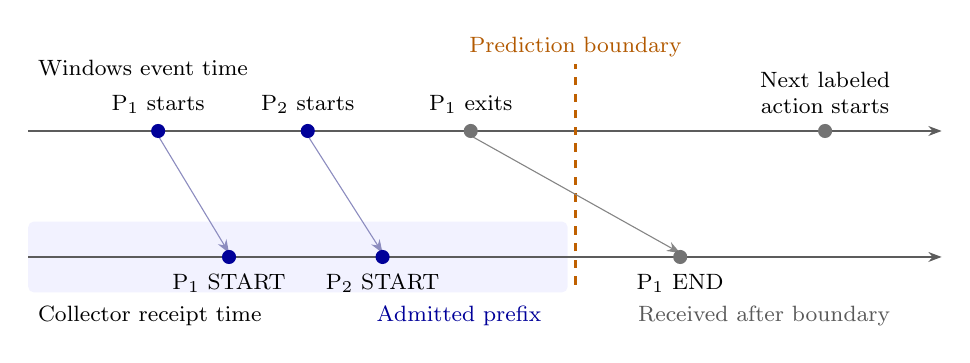
\begin{tikzpicture}[x=1cm,y=1cm,>=Stealth,
  event/.style={circle,inner sep=1.8pt,fill=blue!60!black},
  later/.style={circle,inner sep=1.8pt,fill=black!55},
  txt/.style={font=\footnotesize,align=center}]
  \fill[blue!5,rounded corners=2pt] (0.5,0.75) rectangle (7.35,1.65);
  \draw[->,black!64] (0.5,2.8) -- (12.1,2.8);
  \draw[->,black!64] (0.5,1.2) -- (12.1,1.2);
  \node[txt,anchor=west] at (0.5,3.6) {Windows event time};
  \node[txt,anchor=west] at (0.5,0.45) {Collector receipt time};
  \draw[thick,orange!75!black,dashed] (7.45,0.85) -- (7.45,3.65);
  \node[txt,text=orange!70!black] at (7.45,3.87) {Prediction boundary};
  \draw[->,blue!44!black!45] (2.15,2.74) -- (3.05,1.25);
  \draw[->,blue!44!black!45] (4.05,2.74) -- (5.0,1.25);
  \draw[->,black!48] (6.12,2.74) -- (8.78,1.25);
  \node[event,label={[txt]above:{P$_1$ starts}}] at (2.15,2.8) {};
  \node[event,label={[txt]above:{P$_2$ starts}}] at (4.05,2.8) {};
  \node[later,label={[txt]above:{P$_1$ exits}}] at (6.12,2.8) {};
  \node[later,label={[txt]above:{Next labeled\\action starts}}] at (10.62,2.8) {};
  \node[event,label={[txt]below:{P$_1$ START}}] at (3.05,1.2) {};
  \node[event,label={[txt]below:{P$_2$ START}}] at (5.0,1.2) {};
  \node[later,label={[txt]below:{P$_1$ END}}] at (8.78,1.2) {};
  \node[txt,anchor=east,text=blue!60!black] at (7.14,0.45) {Admitted prefix};
  \node[txt,anchor=west,text=black!65] at (8.12,0.45) {Received after boundary};
\end{tikzpicture}
\caption{A schematic prediction boundary. P$_1$ and P$_2$ denote two
observed processes. The predictor receives both START records before
the boundary. The END of P$_1$ arrives afterward even though P$_1$ has
already exited. The next attacker action supplies the evaluation label.}
\label{fig:cutoff}
\end{figure}

Figure~\ref{fig:cutoff} shows why availability cannot be reconstructed
from occurrence time alone: P$_1$ has already exited, yet its result is
not part of the admitted prefix. A later receipt can change later
forecasts but leaves the earlier prefix intact.

\section{Benign workloads and evaluation conditions}
\label{sec:conditions}

Some executions run benign tasks on the same host while the source
procedure executes. Three benign workers are defined. Worker~A repeats a
read-only \texttt{where} search, a \texttt{tasklist} process listing, and
an \texttt{sc} service listing every 1,200~ms in a separate scratch
directory. Worker~B repeats a \texttt{dir /b} directory listing and a
\texttt{certutil} SHA-256 hash of a scratch file at a fixed 1,200~ms
interval. Worker~C lists services with \texttt{sc} and then the local
interfaces with \texttt{ipconfig /all} at a fixed 2,400~ms interval; it
makes no external connection. A worker starts before the source is
dispatched and stops after the source finishes. It does not read the
source's actions, results, or requests, nor the defender's receipts,
and the source keeps its own result-dependent choice of actions. The
benign processes therefore enter the received stream without taking
part in the source's decisions. We call a condition with at least one
benign worker a \emph{background condition}.
Table~\ref{tab:conditions} lists the conditions and the two placements
of the file targets.
% 근거: RECORD:34--42; PAPER_DEFINITIONS.md §1.

\begin{table}[htbp]
\centering
\caption{Evaluation conditions and target layouts. ``C-fold FIT'' states
whether the condition's benign work occurs in the 603 training runs of
the C-fold (Section~\ref{sec:conditions}).}
\label{tab:conditions}
\begin{tabularx}{\textwidth}{@{}llX@{}}
\toprule
Identifier & C-fold FIT & Definition \\
\midrule
\texttt{ORIGINAL\_18} & seen & Original source procedure without a benign worker; all 18 actions \\
\texttt{C\_ONLY} & unseen & Source procedure with worker C \\
\texttt{A+C} & unseen & Source procedure with workers A and C \\
\texttt{B+C} & unseen & Source procedure with workers B and C \\
\midrule
\texttt{FLAT} & --- & Four file targets \texttt{echo}, \texttt{foxtrot}, \texttt{golf}, \texttt{hotel} placed as sibling directories \\
\texttt{NESTED} & --- & As \texttt{FLAT}, except that \texttt{foxtrot} is moved under \texttt{echo}; \texttt{echo} remains a target, and the two payloads have different search roots \\
\bottomrule
\end{tabularx}
\end{table}
% 표 기호: 본문·표의 조건 이름은 A+C FLAT, A+C NESTED, C_ONLY, B+C,
% ORIGINAL_18로 통일한다(개요 전체 규칙). 원고의 "C-only"는 C_ONLY로 바꿨다.
% TODO(사람): 배치 FLAT/NESTED는 A+C에서만 따로 보고됩니다. C_ONLY와 B+C
% 실행은 어느 배치를 쓰는지, 그리고 FIT 603실행에 NESTED 배치가 들어 있는지
% 알려 주세요. 표의 "---"를 채울 수 있습니다.

All new experiments in this thesis train on the C-fold, the outer fold
in which every variant of worker~C is withheld from the training runs.
We call these 603 runs the \emph{FIT set}. A condition is \emph{seen}
if its benign work occurs in the FIT set and \emph{unseen} otherwise;
under the C-fold, every condition that contains worker~C is unseen, and
\texttt{ORIGINAL\_18} is the seen reference. The B-fold withholds
worker~B instead. It appears only in the older comparisons of
Appendix~\ref{app:secondary-results} and is not used for any result in
the main chapters.
% 근거: RECORD:44; answers.md 7-(2). 이 정의로 05_evaluation.tex의 기존 TODO
% ("define the B-fold and C-fold")의 fold 부분을 닫는다. 그 TODO의 natural
% 전달 일정 정의는 [직접 기입]으로 남는다. 05장을 쓸 때 TODO를 정리해 주세요.

The C-fold makes the difference between seen and unseen conditions
concrete. Worker~C runs \texttt{ipconfig /all}, and the input
represents such records as an IP hint. Of the 4,824 boundaries in the
FIT set, 2,425 had received at least one IP hint. These hints came from
658 distinct native records in 329 runs, and all 658 belong to the
process lineage of the attack procedure. In the 60 \texttt{A+C}
development runs (660 rows), all 353 native records carrying an IP hint
belong instead to the lineage of benign worker~C. The same kind of
evidence is thus produced by the attacker during training and by benign
work at evaluation. Lineage was determined from audit information that
the model never receives. We use this case to show what a condition
unseen in training looks like; the audit does not establish it as the
cause of any seed's success or failure.
% 근거: ORIG:PROPHET_REL_GLOBAL_SEED_POPULATION_20261118/FINAL_REPORT_KO.md:9.
% 60실행·660행 = A+C FLAT 31·341 + NESTED 29·319 (같은 파일, 135실행 개발 집합).
% 4,824는 원 파일의 "자연 경계" 수다. natural boundary의 정의는 5장 [직접 기입].
% TODO(사람): "IP hint"가 ipconfig 사건에서 만든 입력 표현이라는 설명이 맞는지
% 확인해 주세요(원 파일은 FIT의 ipconfig.exe START/END 880개가 모두 공격
% 계보라고 적는다).

\section{A recorded file-processing decision}
\label{sec:recorded-case}

Table~\ref{tab:recorded-case} shows part of the received prefix for
execution \texttt{THME0064}, from the three-target development set,
before its first file-processing decision (\texttt{SEQ\_5}). The path
names distinguish three synthetic targets. The marker concerns
\texttt{alpha}, whose earlier payload search returned a nonzero exit
status, while the marker's own zero exit status belongs to a different
process. Within the \texttt{alpha} group, the latest received result is
therefore a success, and the search result comes from an earlier record.
Grouping the records by target lets a model read the two processes
together while keeping their results apart. The next recorded action
was a synthetic file search. The example previews the mechanism examined
in Chapter~\ref{ch:diagnosis}, where the in-house seed instability is
traced to the lookup of the current target's earlier result.

\begin{table}[htbp]
\centering
\caption{Selected records received before the decision in
\texttt{THME0064}. Rows show the observed target groups. For the
two other targets, only the search termination is shown.}
\label{tab:recorded-case}
\begin{tabularx}{\textwidth}{@{}llX@{}}
\toprule
Target group & Record ID & Evidence available before the decision \\
\midrule
\texttt{bravo}, \texttt{charlie} & & Payload search END at each target, zero exit status \\
\texttt{alpha} & 207481 & Payload search END, nonzero exit status \\
\texttt{alpha} & 207483 & Marker START \\
\texttt{alpha} & 207485 & Marker END, zero exit status \\
\bottomrule
\end{tabularx}
\end{table}
% 기존 원고의 target-wise GRU 대 relation attention 확률 비교 문장
% (0.434/0.450/0.481, 0.984/0.483/0.517)은 개요에 따라 부록 B.5로 옮긴다.
% 부록 B를 쓸 때 그 문장과 함께 "target-wise GRU: [직접 기입]" 자리를 남긴다.
% 기존 sec:membership 참조는 이 장에서 뺐다(소속 교환 설명은 부록 B에서 한 번만).

% ---------------------------------------------------------------
% 사람에게 물을 것 (3장)
% 1. UNKNOWN 상태의 범위: 결속되지 않은 END·대상 미배정 record만인지,
%    END가 아직 수신되지 않은 START의 결과도 UNKNOWN으로 부르는지.
% 2. FLAT/NESTED 배치가 C_ONLY, B+C 실행과 FIT 603실행에 어떻게 들어가는지
%    (표 tab:conditions의 "---" 칸).
% 3. "IP hint"의 정의: ipconfig 사건에서 만든 입력 표현이 맞는지.
% 4. THME0064가 속한 3대상 개발 집합이 C-fold FIT로 학습한 모델로 평가된
%    것인지(6장 기제 예고 문장의 범위 확인).
% ---------------------------------------------------------------

\chapter{Baseline Predictor and Consensus Distillation}
\label{ch:method}
% 개요 4장. 다시 썼다. 옛 EVENT GRU/flat/THM/REL/Local History/확률 평균/
% 빈도 기준선의 정의, 식 eq:eventgru·eq:relation·eq:mixture·eq:table, 그림
% fig:model은 4.2절의 요약과 부록 B로 옮긴다(개요 13장 B.1, B.5). 질문 A3의 답이
% 없어 fig:model은 이 장에 두지 않는다. 그림의 TikZ 원본은 커밋 28c02eb의 이
% 파일에 있다. 부록 B를 다시 쓸 때 fig:model, eq:mixture, eq:table 라벨을 그쪽에
% 살려야 b_supplemental_results.tex의 기존 참조가 깨지지 않는다.

A CD student and the baseline predictor, REL\_GLOBAL, share one
architecture and differ only in the loss used during training. We
first describe REL\_GLOBAL and then the added loss term, the choice of
teachers, the names of the trained groups used in later chapters, and
what was changed when the method was moved to ADS-24 and to three
general encoders.

\section{The baseline predictor}
\label{sec:method-baseline}

REL\_GLOBAL maps the received prefix $X_t$ of
Equation~\ref{eq:receipt} to a distribution over the 18 actions. Its
parts are an event encoder, an event-level recurrent state, a relational
residual, and an output head (Figure~\ref{fig:relglobal}).

% 그림: REL_GLOBAL 구조(5.1절). 2026-11-25 추가. 수치는 5.1절 식 eq:event-enc, eq:head, eq:relation-attn 과 같다.
% 교차 검토 1차(독립 에이전트) 반영: 캡션 범위, 관계 잔차 두 단계, 벌점은 e_i 에, age·r 출처, 라벨 크기.
\begin{figure}[tb]
\centering
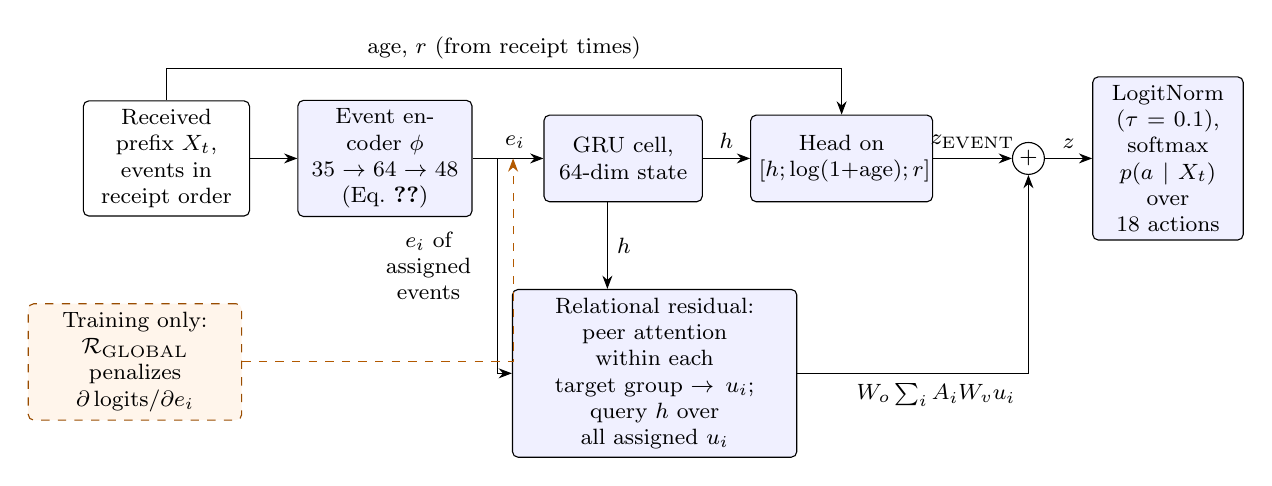
\begin{tikzpicture}[>=Stealth,node distance=4mm and 6mm,
  box/.style={draw,rounded corners=2pt,align=center,font=\footnotesize,
    minimum height=11mm,inner sep=3pt,fill=white},
  main/.style={box,fill=blue!6},
  aux/.style={box,fill=orange!8,draw=orange!60!black,dashed},
  lab/.style={font=\footnotesize,align=center}]
  \node[box,text width=19mm] (in) {Received prefix $X_t$,\\events in\\receipt order};
  \node[main,text width=20mm,right=of in] (enc) {Event encoder $\phi$\\$35\to64\to48$\\(Eq.~\ref{eq:event-enc})};
  \node[main,text width=18mm,right=9mm of enc] (gru) {GRU cell,\\64-dim state};
  \node[main,text width=21mm,right=of gru] (head) {Head on\\$[h;\log(1{+}\mathrm{age});r]$};
  \node[circle,draw,inner sep=1pt,font=\footnotesize,right=10mm of head] (plus) {$+$};
  \node[main,text width=17mm,right=6mm of plus] (ln) {LogitNorm\\($\tau=0.1$), softmax\\$p(a\mid X_t)$ over\\18 actions};
  \node[main,text width=34mm,below=11mm of gru,xshift=4mm] (rel)
    {Relational residual:\\peer attention within each\\target group $\to u_i$;\\query $h$ over all assigned $u_i$};
  \node[aux,text width=25mm,below=11mm of in,xshift=-4mm] (pen)
    {Training only:\\$\mathcal{R}_{\mathrm{GLOBAL}}$ penalizes\\$\partial\,$logits$/\partial e_i$};
  \draw[->] (in) -- (enc);
  \draw[->] (enc) -- coordinate[pos=0.35] (ei) node[lab,above,pos=0.6]{$e_i$} (gru);
  \draw[->] (gru) -- node[lab,above]{$h$} (head);
  \draw[->] (head) -- node[lab,above]{$z_{\mathrm{EVENT}}$} (plus);
  \draw[->] (plus) -- node[lab,above]{$z$} (ln);
  \draw[->] (ei) |- node[lab,left,pos=0.25,text width=15mm]{$e_i$ of\\assigned\\events} (rel.west);
  \draw[->] ([xshift=-2mm]gru.south) -- node[lab,right]{$h$} ([xshift=-2mm]gru.south |- rel.north);
  \draw[->] (rel.east) -| node[lab,below,pos=0.3]{$W_o\sum_i A_i W_v u_i$} (plus.south);
  \draw[->,dashed,orange!70!black] (pen.east) -| ([xshift=2mm]ei);
  \draw[->] (in.north) -- ++(0,4mm) -| node[lab,above,pos=0.25]{age, $r$ (from receipt times)} (head.north);
\end{tikzpicture}
\caption[REL\_GLOBAL, the baseline predictor]{REL\_GLOBAL, the baseline predictor and the architecture of every
in-house CD student; the students of Chapter~\ref{ch:generality} keep their
own encoders. Solid arrows are the inference path. The dashed box and arrow
mark the representation-gradient penalty on the event vectors $e_i$, used
only in training. Events without an assigned target stay in the recurrent
path but not in the relational residual, and an empty prefix uses a learned
initial state.}
\label{fig:relglobal}
\end{figure}


\paragraph{Event encoder.} Each admitted event is first described by a
35-dimensional vector: an 8-dimensional embedding of the image name,
the mean of 8-dimensional embeddings of the normalized command tokens
(a zero vector for an empty command), an 8-dimensional embedding of the
observed-command hint (with a NONE value), a 4-dimensional START/END
type embedding, a 4-dimensional status embedding, and three numbers,
$\log(1+\Delta_{\mathrm{native}})$, $\log(1+\Delta_{\mathrm{receipt}})$
and a link indicator. Here $\Delta_{\mathrm{native}}$ is the event's
native time minus the earliest native time in the prefix and
$\Delta_{\mathrm{receipt}}$ is the cutoff minus the event's receipt
time, both in seconds and clipped at zero. The status vocabulary is
UNOBSERVED, UNMATCHED, ZERO, NONZERO, STATUS\_MISSING and
STATUS\_MALFORMED (Section~\ref{sec:receipt}). The vector is mapped to
48 dimensions by
\begin{equation}
  e_i=\phi(v_i)=\mathrm{LayerNorm}\bigl(W_2\,\mathrm{GELU}(W_1 v_i)\bigr),
  \qquad W_1\in\mathbb{R}^{64\times 35},\; W_2\in\mathbb{R}^{48\times 64}.
  \label{eq:event-enc}
\end{equation}
All vocabularies are fitted on FIT data only. The command-token
vocabulary holds at most 1,024 tokens, in order of frequency, plus
padding and unknown entries.
% 출처: inputs/data/original_reports/lab/DIVERSE3K_20261027/COMMAND_REPRESENTATION_20261028/PRE_SPEC_V1.md:13
%   ("train 정규화 명령에서만 빈도순 … 최대 1,024개 … PAD/UNK"; sources/atlas_answers/repro.md:77).
The vocabularies and normalizers are those
fitted on the original 404 FIT runs and are kept fixed for every
extension of FIT; tokens that occur only in the added runs map to the
unknown entry.

\paragraph{Recurrent state and head.} Events enter a gated recurrent
unit cell~\cite{cho2014gru} with a 64-dimensional state, one event per
step in receipt order.
% 원문: Cho et al. (EMNLP 2014) §2.3 p.3, reset·update 게이트를 가진 "new type of hidden unit".
 The head is
\begin{equation}
  z_{\mathrm{EVENT}}=W_4\,\mathrm{GELU}\bigl(W_3[h;\,\log(1+\mathrm{age});\,r]\bigr),
  \qquad W_3\in\mathbb{R}^{64\times 66},\; W_4\in\mathbb{R}^{18\times 64},
  \label{eq:head}
\end{equation}
where $h$ is the last state, age is the time since the last receipt and
$r$ indicates whether anything has been received. An empty prefix uses a
learned initial state with age and $r$ set to zero.

\paragraph{Relational residual.} Let $a_i$ be the target that the
parser assigns to event $i$, and let $M_{ij}=1$ when events $i$ and $j$
are both assigned and $a_i=a_j$ (including $i=j$). Events that match
several target paths ambiguously or none are left unassigned. With
shared key and value maps $W_k$ and $W_v$,
\begin{equation}
  P_{ij}=\operatorname*{softmax}_{j:\,M_{ij}=1}
    \frac{(W_{\mathrm{peer}}e_i)^{\top}W_k e_j}{\sqrt{48}},\quad
  u_i=e_i+\sum_j P_{ij}W_v e_j,\quad
  A_i=\operatorname*{softmax}_{i}\frac{(W_q h)^{\top}W_k u_i}{\sqrt{48}},
  \label{eq:relation-attn}
\end{equation}
and the logits are $z=z_{\mathrm{EVENT}}+W_o\sum_i A_iW_v u_i$, where
the sums run over assigned events. $W_o$ is initialized to zero. When no
event is assigned, $z=z_{\mathrm{EVENT}}$. Unassigned events stay in the
recurrent path but do not enter the residual, so the result recorded for one target is
read together with that target's other records and kept apart from the
results of the others. The model has 59,882 parameters.
% 출처: OT/THM_RELATION_AWARE_ATTENTION_FIXED_20261108/CONTRACT.md:14 ("unmatched events do not
% enter the residual read but remain in the original EVENT path"). 10회차 방법 P1-1: status 가
% UNOBSERVED 인 사건을 잔차에서 뺀다는 근거는 계약에 없어 그 구절을 지웠다(2026-11-24, Claude).

\paragraph{LogitNorm.} Wei et al.\ define LogitNorm as a training
loss: the cross-entropy is computed on logits normalized to a fixed
norm~\cite{wei2022mitigating}. We use a variant inspired by it that
% 원문: Wei et al. (ICML 2022) §3.2 식 (3)–(4) p.3 "the logit vector is normalized to be a unit vector with a constant magnitude".
applies the same normalization in training and at inference, replacing
$z$ by $z/[\tau\max(\|z\|_2,10^{-8})]$ with $\tau=0.1$, with the gradient
flowing through the denominator; applying it at inference is our
choice, not part of the cited method. It limits how far the training
loss can be lowered by inflating the logits. In this thesis
\emph{LogitNorm} refers to this train-and-inference variant.

\paragraph{Representation-gradient penalty.}
$\mathcal{R}_{\mathrm{GLOBAL}}$ is a representation-gradient penalty
inspired by input-gradient regularization~\cite{ross2017improving}:
Ross and Doshi-Velez penalize the gradient with respect to the model
input, whereas $\mathcal{R}_{\mathrm{GLOBAL}}$ differentiates with
respect to the internal 48-dimensional event representations. During
training only, for each FIT occurrence, the audit-known worker roles
set a count, the
% 원문: Ross & Doshi-Velez (AAAI 2018) 'Input Gradient Regularization' 절 식 (6) p.3, 목적함수 H(y, y_hat) + lambda * ||grad_x H(y, y_hat)||_2^2.
number $k$ of worker events; the penalty then draws exactly $k$ events
at random from all received events, so it does not target the worker
events themselves. An earlier variant that penalized only the worker events showed no
advantage over this random draw (Table~\ref{tab:rej-candidates},
row~7). Where the count is zero, no penalty is applied. For each drawn event it takes the
squared gradient, with respect to that event's 48-dimensional vector
$e_i$, of a single Rademacher projection of the centered 18-way logits;
this is an unbiased estimate of the squared Frobenius norm of the
Jacobian. The penalty is averaged over the drawn events and then over
occurrences. It therefore discourages logits that change sharply with one
event's representation.

The model was reached in steps. REL, an earlier relation model, added
the residual of Equation~\ref{eq:relation-attn} to the event-level
predictor. At that earlier stage, on 64 new runs (512 rows) from 16
held-out configurations and averaged over three seeds, it lowered the
mean NLL of the same predictor without a relation path, EVENT GRU,
from 0.217 to 0.046, and a control that exchanged target membership
between groups showed that the gain came from which records belong to
which target (Appendix~\ref{app:secondary-results}). Those models were
trained on other data and are not comparable with later chapters, and
no criterion of this thesis tests the residual. REL was then trained
on the 603-run C-fold FIT set, which includes the benign-worker runs,
for 1,346 updates. LogitNorm was then
added (REL\_NORM), and finally $\mathcal{R}_{\mathrm{GLOBAL}}$ with
coefficient 0.1. The parameter count stayed at 59,882 throughout.
% 2026-11-26 본문 분량: 옛 4.2절 "Evidence for the relational residual"을 이 문단으로 줄였다.
%   근거: ORIG:THM_RELATION_VALUE_FOLLOWUP_FIXED_20261109/REPORT_KO.md:11,18,23 (EVENT 0.217124 → REL 0.045797,
%   seed 11/29/47, 새 64실행·512행, 16개 보류 구성); 소속 교환 0.058365 → 0.086855 는 부록 B.3.
Appendix~\ref{app:repro} states which code and records exist and which
are not in the archive available to us; the thesis does not supply
everything needed to repeat the in-house experiments
(Section~\ref{sec:repro-code}).
% 출처: sources/atlas_answers/repro.md 6번·7번.
% 사건 표현 35차원·φ·head: atlas OTL/RECEIPT_BATCH_METHOD_DECISION_20261101/SELECTED_METHOD_CONTRACT.md:18;
%   OT/EVENT_CONTEXT_READOUT_PREFIT_20261105/CURRENT_REPRESENTATION_AUDIT_KO.md:14,17.
% status 어휘: SELECTED_METHOD_CONTRACT.md:11,18. 어휘 1,024: OTL/DIVERSE3K_20261027/COMMAND_REPRESENTATION_20261028/PRE_SPEC_V1.md:13.
% 404-only: OT/EXPOSURE_404_VS_476_COMMON_VOCAB_FIXED_20261110/CONTRACT.md:5.
% 미배정 -1: OT/V3_MEMORY_EXTERNAL_METHODS_FIXED_20261106/METHOD_SPEC_KO.md:9.
% 관계 잔차 식: OT/THM_RELATION_AWARE_ATTENTION_FIXED_20261108/CONTRACT.md:14,16-19;
%   OT/REL_PEER_HISTORY_FACTORIAL_FIXED_20261110/CONTRACT.md:3 (공유 key/value, √48, self-edge, 0 초기화).
% 59,882: OT/EXPOSURE_404_VS_476_COMMON_VOCAB_FIXED_20261110/REPORT_KO.md:11.
% LogitNorm 학습·추론: OT/SLOT_LOCAL_BITA_LOGITNORM_CONFIRM_20261116/CONTRACT.md:17;
%   OT/SLOT_SERIAL_HARD_REL_NORM_FIXED_20261116/CONTRACT.md:3.
% R_GLOBAL: OT/PROPHET_WORKER_GLOBAL_COUNT_MATCH_20261117/FINAL_REPORT_KO.md:10,11;
%   OT/PROPHET_WORKER_INPUT_GRAD_FIXED_20261117/FINAL_REPORT_KO.md:9;
%   OT/PROPHET_BITA_GLOBAL_COUNT_INTERACTION_20261118/FINAL_REPORT_KO.md:8 (48차원 EVENT 표현).
% 계보: OT/REL_EVIDENCE_PRESERVING_COMPARISON_20261113/FINAL_REPORT_KO.md:26,28;
%   OT/SLOT_SERIAL_HARD_REL_NORM_FIXED_20261116/CONTRACT.md:3; OT/PROPHET_WORKER_INPUT_GRAD_FIXED_20261117/FINAL_REPORT_KO.md:7.
% "Δ의 정확한 단위·절단": 원 계약의 log1p((native−min_native_prefix)+/1s), log1p((cutoff−receipt)+/1s).

Training uses the 603 runs of the FIT set
(Section~\ref{sec:conditions}). The objective is
\begin{equation}
  \mathcal{L}_{\mathrm{base}}
  = \mathcal{L}^{\mathrm{FIT}}_{\mathrm{CE}}
  + 0.1\,\mathcal{R}_{\mathrm{GLOBAL}},
  \label{eq:base-loss}
\end{equation}
where $\mathcal{L}^{\mathrm{FIT}}_{\mathrm{CE}}$ is the 18-way action
cross-entropy with each FIT run given equal weight. Each update takes
32 FIT occurrences drawn from successive random permutations of the 603
runs. An occurrence holds all natural boundaries of one run together
with the same boundaries under one of its 16 delayed schedules
(Section~\ref{sec:task-rows}); the loss is averaged within the run,
and the 32 occurrences are weighted equally. Each model is
trained for 1,346 such updates with AdamW~\cite{loshchilov2017decoupled}
(weight decay 0.01, gradient clipping at 2), and the learning rate
follows a cosine schedule from 0.002 to 0.0002. The last checkpoint is
% 원문: Loshchilov & Hutter (ICLR 2019) §2 p.3 "our variant of Adam with decoupled weight decay (AdamW)" (Algorithm 2).
kept; no checkpoint is selected by a validation score. All 30 seeds of
a group share this procedure and differ only in the seed as
defined in Chapter~\ref{ch:introduction}. Section~\ref{sec:repro-training} lists the seeds and the remaining
training settings.
% 근거: RECORD:151; PAPER_DEFINITIONS.md §2 (실행 동등 18-way CE, 계수 .1의
% GLOBAL_COUNT_MATCH, weight decay .01, clip 2, 마지막 checkpoint).
% 출처(occurrence 표집): atlas OTL/RECEIPT_BATCH_METHOD_DECISION_20261101/SELECTED_METHOD_CONTRACT.md:34;
%   OT/AUX_MOE3_PAPER_METHOD_RESULTS_20261104/PAPER_METHOD_RESULTS_KO.md:32 (복원추출, 중복 유지);
%   OT/EXPOSURE_404_VS_476_COMMON_VOCAB_FIXED_20261110/CONTRACT.md:4 (repro.md 6-(8)).
% 출처(표집기 구현, 위 atlas 계약의 "복원추출"을 대신함): 원래 PC: REL_EVIDENCE_PRESERVING_COMPARISON_20261113/fit_data.py:67
%   (torch.randperm(len(runs),generator=gen); manual_seed(seed+99237); 일정 index = 뽑힌 횟수 mod 16);
%   원래 PC: PROPHET_ENV_CONSENSUS_KD_V3_20261120/fit_v3.py:53 (REL_GLOBAL 이후 계보도 이 trace를 쓴다).

% 2026-11-26: 옛 4.2절(sec:method-relation-evidence)은 4.1절 끝 문단과 부록 B 로 옮겼다.
% 9회차 문장 P2-4: 소속 교환 대조의 모델은 THM이다(atlas THM_GROUP_BINDING_FIXED_20261108 결론,
%   "정확한 대상 그룹으로 학습한 THM ... 0.058365 대 0.086855"). 부록 B와 맞췄다.
% 근거: ORIG:THM_RELATION_VALUE_FOLLOWUP_FIXED_20261109/REPORT_KO.md:11,18,23
% (EVENT 0.217124 → REL 0.045797, 89.06% → 97.98%, FIT 476 확장, 900 update,
% seed 11/29/47, 새 64실행·512행, 16개 보류 구성). 소속 교환 0.058365 →
% 0.086855, FIT 436, 이미 열람한 127실행·508행, 3 seed(개요 C표의 대조).
% 소속 교환 대조의 설명은 부록 B.3에서 한 번만 한다.
% 계보(REL → hard REL → REL_NORM → REL_GLOBAL)는 4.1절 끝에 넣었다(repro.md 7번).

\section{Consensus distillation}
\label{sec:method-cd}

A CD student has the architecture of REL\_GLOBAL and no additional
parameters, so at inference it is the same single model. What changes
is the training loss; Figure~\ref{fig:cd} shows the whole procedure. Let $J$ be a fixed set of \emph{teachers},
trained REL\_GLOBAL models whose weights are frozen, and let $p_j$ be
the predicted distribution of teacher $j$ at temperature~1. On an
unlabeled input $x$ from the target environment, the target is the
arithmetic mean of the teachers' probabilities, and the student
$p_\theta$ is pulled toward it by a Kullback--Leibler term:
\begin{equation}
  \bar{p}_J(a\mid x)=\frac{1}{|J|}\sum_{j\in J}p_j(a\mid x),
  \qquad
  \mathrm{KL}\bigl(\bar{p}_J \,\|\, p_\theta\bigr)(x)
  =\sum_{a=1}^{18}\bar{p}_J(a\mid x)
   \log\frac{\bar{p}_J(a\mid x)}{p_\theta(a\mid x)} .
  \label{eq:cd-target}
\end{equation}
The divergence runs from the teachers to the student, so the student is
penalized most where the teachers place probability that it does not.
The student's loss keeps both terms of Equation~\ref{eq:base-loss} and
adds this divergence with coefficient 0.25:
\begin{equation}
  \mathcal{L}
  = \mathcal{L}^{\mathrm{FIT}}_{\mathrm{CE}}
  + 0.1\,\mathcal{R}_{\mathrm{GLOBAL}}
  + 0.25\,\mathrm{KL}\bigl(\bar{p}_J \,\|\, p_\theta\bigr)_{\mathrm{env}} ,
  \label{eq:cd-loss}
\end{equation}
where the subscript denotes the mean over the unlabeled environment
rows of the update. Each update adds 32 such rows to its 32 labeled FIT
occurrences; no label, run identifier, or source and worker
membership of these rows enters the loss. The distillation temperature
is unrelated to the LogitNorm temperature $\tau$: the student still
trains with LogitNorm at $\tau=0.1$, and the teacher target is taken at
temperature~1 without further rescaling. As
Section~\ref{sec:related-distillation} notes, the computation is
knowledge distillation toward the average of several
models~\cite{hinton2015distilling}. Unlike ensemble distribution
distillation~\cite{malinin2019ensemble}, the target is the plain mean
and carries no model of the spread among teachers.
% 원문: Hinton et al. arXiv:1503.02531 §2 "arithmetic or geometric mean of their individual predictive
%   distributions as the soft targets"; Malinin et al. arXiv:1905.00076 초록 "distilling the distribution
%   of the predictions from an ensemble, rather than just the average prediction". 확인됨.
% 근거: RECORD:130--139, 153; PAPER_DEFINITIONS.md §2 (q_J 식, KL 방향 교사‖학생,
% 구현 F.kl_div(log_softmax(student), teacher_prob).sum(-1).mean(), 계수 .25,
% update당 무라벨 32행, "LogitNorm 0.1은 증류 온도 1과 별개").

% 그림: CD 흐름(5.3–5.5절). 2026-11-25 추가. 숫자는 5.3절 eq:cd-loss, 5.4절 교사 선정, 5.5절 tab:variants 와 같다.
% 교차 검토 1차 반영: 자체 실험실 KD_ALL 의 경우로 범위를 밝히고, 적응 입력(배경 119 + seen 48), 교사도 같은 행을 봄,
%   FIT 쪽은 CE 와 R_GLOBAL, 식 줄바꿈. A+C 개발 실행은 배경 입력 119실행 안에 있다(04_method sec:method-teachers, 4.6절).
\begin{figure}[tb]
\centering
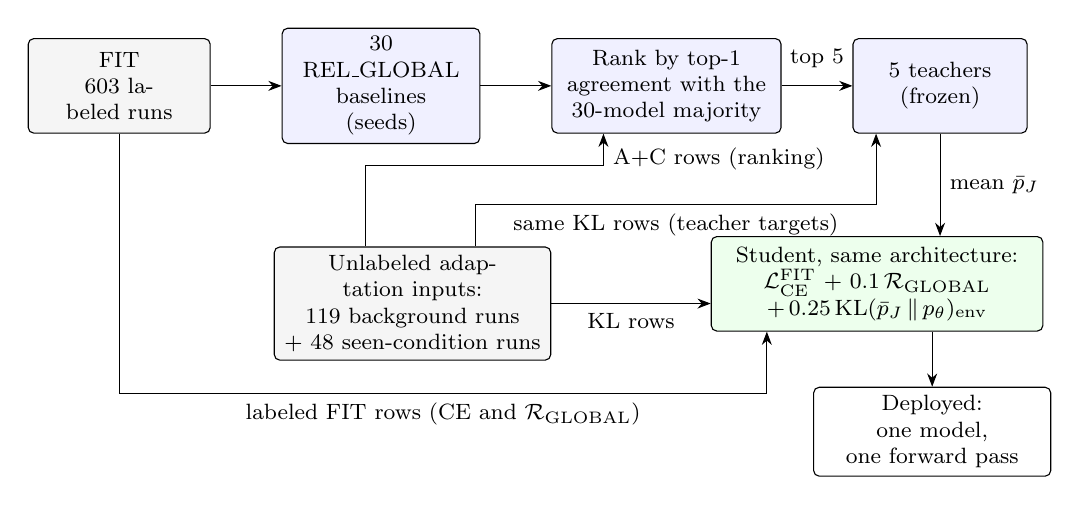
\begin{tikzpicture}[>=Stealth,node distance=5mm and 9mm,
  box/.style={draw,rounded corners=2pt,align=center,font=\footnotesize,
    minimum height=12mm,inner sep=3pt},
  data/.style={box,fill=black!4},
  model/.style={box,fill=blue!6},
  stud/.style={box,fill=green!7},
  lab/.style={font=\footnotesize,align=center}]
  \node[data,text width=21mm] (fit) {FIT\\603 labeled runs};
  \node[model,text width=23mm,right=of fit] (base) {30 REL\_GLOBAL\\baselines\\(seeds)};
  \node[model,text width=27mm,right=of base] (rank) {Rank by top-1\\agreement with the\\30-model majority};
  \node[model,text width=20mm,right=of rank] (teach) {5 teachers\\(frozen)};
  \node[data,text width=33mm,below=13mm of base,xshift=4mm] (env)
    {Unlabeled adaptation inputs:\\119 background runs\\$+$ 48 seen-condition runs};
  \node[stud,text width=40mm,below=13mm of teach,xshift=-8mm] (stu)
    {Student, same architecture:\\$\mathcal{L}^{\mathrm{FIT}}_{\mathrm{CE}}+0.1\,\mathcal{R}_{\mathrm{GLOBAL}}$\\$+\,0.25\,\mathrm{KL}(\bar p_J\,\|\,p_\theta)_{\mathrm{env}}$};
  \node[box,text width=28mm,minimum height=8mm,below=7mm of stu,xshift=7mm] (dep) {Deployed: one model,\\one forward pass};
  \draw[->] (fit) -- (base);
  \draw[->] (base) -- (rank);
  \draw[->] (rank) -- node[lab,above,yshift=1mm]{top 5} (teach);
  \draw[->] ([xshift=-6mm]env.north) |- ([xshift=-8mm,yshift=-4mm]rank.south) -- node[lab,right,pos=0.2]{A+C rows (ranking)} ([xshift=-8mm]rank.south);
  \draw[->] ([xshift=8mm]env.north) |- node[lab,below,pos=0.75]{same KL rows (teacher targets)} ([xshift=3mm,yshift=-9mm]teach.south west) -- ([xshift=3mm]teach.south west);
  \draw[->] (teach.south) -- node[lab,right]{mean $\bar p_J$} (teach.south |- stu.north);
  \draw[->] (env.east) -- node[lab,below]{KL rows} (env.east -| stu.west);
  \draw[->] (fit.south) -- ++(0,-33mm) -| node[lab,below,pos=0.25]{labeled FIT rows (CE and $\mathcal{R}_{\mathrm{GLOBAL}}$)} ([xshift=-14mm]stu.south);
  \draw[->] ([xshift=7mm]stu.south) -- (dep.north);
\end{tikzpicture}
\caption[Consensus distillation as run in-house for KD\_ALL]{Consensus distillation as run in-house for KD\_ALL
(Section~\ref{sec:method-variants}). Thirty baselines
are trained on FIT and ranked by their agreement, own vote included, with the
30-model majority on unlabeled A+C rows; the five most agreeing become frozen
teachers. The student keeps the baseline loss on FIT and follows the
teachers' mean probability on the same unlabeled adaptation rows. At
inference it is one model of the baseline's size. On ADS-24 and for the
general encoders the teachers are chosen again in each setting
(Section~\ref{sec:method-transfer}).}
\label{fig:cd}
\end{figure}


\section{Teacher selection}
\label{sec:method-teachers}

The unlabeled background inputs are the 119 background runs (1,309
rows) of the 135-run development set (Section~\ref{sec:conditions}),
and teachers are ranked on its 60 A+C runs (660 rows).
Teachers are chosen from 30 REL\_GLOBAL seeds trained with
Equation~\ref{eq:base-loss}. For each row of these unlabeled A+C inputs,
the 30 models vote with their top-1 actions, and the majority action
serves as the reference. Each model's own vote is included.
A model's
\emph{top-1 agreement} is the fraction of rows on which its top-1
action equals that majority, computed within each run and then averaged
over runs with equal weight. The five models with the highest agreement
form $J$; Section~\ref{sec:repro-training} gives the tie rules.
% 출처(열 순서): 원래 PC: INDEPENDENT_POLICY_LAB_20261026/RECEIPT_BATCH_METHOD_DECISION_20261101/run_receipt_atomic_v2.py:70
%   (labels = checkpoint["candidate_actions"]); 같은 폴더 receipt_atomic_model_v2.py:55;
%   같은 폴더 PREPROCESSOR_V2.json:280 (저장된 18열, 행동 ID 알파벳순).
% 출처(다수결 동률): 원래 PC: ARCH_GENERALITY_STAGE1_20261122/predict_stage1.py:232 (majority = votes.argmax(0)).
The five selected are the teachers of KD\_ENV\_TOP5 and KD\_ALL in
the v2 and v3 rounds (Table~\ref{tab:round-summary} lists the rounds);
the ranking is not
the agreement estimator of Baek et al.~\cite{baek2022agreement}
(Section~\ref{sec:related-underspec}).
% 원문: Baek et al. NeurIPS 2022 §4 ALine-S/ALine-D(짝별 일치도 선). 본문은 관계 설명만 넘긴다. 확인됨.

The rule uses no labels, but it was fixed while we were studying development
runs that had already been inspected, so the teacher choice is not
blind. For REL\_GLOBAL no round compared it with other teacher sets.
For the plain GRU the final checks did (Section~\ref{sec:gen-teachers}):
in the lab the five most agreeing teachers gave the best students of the
sets tried, while on ADS-24 five random teachers did better.
% 2026-11-26 패널 7회차 문체 P1-1·참신성 P1-1: 10.3절 결과와 어긋나던 "비교한 적이 없다"를 고쳤다.
% 근거: PAPER_DEFINITIONS.md §2 "고정 상위 5개 교사 선정". 상위 5 seed는
% 50572, 91513, 71556, 68498, 37406. 입력은 이미 열람한 A+C FLAT·NESTED.
% 다수결 동률은 낮은 행동 열 index, 순위 동률은 낮은 seed. 후보 자신의 표 포함.
% 5회차 방법 리뷰 P3: 동률 규칙을 본문에 옮기고 부록 E의 seed 목록을 가리켰다.
% 출처(열 순서): defs.md 38번; PAPER_DEFINITIONS.md:44; 행동별 표 세 곳의 순서가 부록 A와 같다.

Agreement is used to choose teachers, not to choose a deployed model.
The single seed ranked first by agreement failed preservation on
ORIGINAL\_18: on the development runs its NLL was 0.109 above the mean of
the 30 seeds, against the preservation limit of $+0.020$
(Section~\ref{sec:eval-criteria}), while
the average of the top five passed it at the cost of running five models
at inference. Distillation is what returns that five-model target to a
single model.
% 근거: ORIG:PROPHET_REL_GLOBAL_SEED_POPULATION_20261118/FINAL_REPORT_KO.md:3,43,47
% (S1 단일 seed 50572의 ORIGINAL_18 NLL .739376, 한도 .650865(모집단 평균
% .630865 + .020), 초과 +.108511; 상위5 결합 .548374로 통과. 135실행 개발 집합).
% ADS-24 ρ=+0.127, p=0.503은 2.3절과 8장에 있어 여기서 되풀이하지 않았다.

\section{Trained groups}
\label{sec:method-variants}

Throughout the thesis, a \emph{CD student} is a student trained with
Equation~\ref{eq:cd-loss} toward the mean of five teachers chosen by
the rule of Section~\ref{sec:method-teachers}. In-house its final form
is KD\_ALL; on ADS-24 and for the general encoders of
Chapter~\ref{ch:generality} the teachers are drawn from the 30 baseline
models of the same encoder and data (Section~\ref{sec:method-transfer}).
Table~\ref{tab:variants} lists the groups that appear in the in-house
rounds of Chapters~\ref{ch:evaluation} and~\ref{ch:results}. All groups
share the FIT procedure of Section~\ref{sec:method-baseline}; they differ
in the teacher set and in the unlabeled inputs of the KL term, which we
call \emph{adaptation inputs}. The
background inputs are 119 runs (1,309 rows) under background conditions.
KD\_ALL adds 48 runs (354 rows) of the seen condition to them, the 16
of the development set and the 32 \texttt{ORIGINAL\_18} runs of an
earlier new-run check (\texttt{OBSERVED\_HEAD},
Section~\ref{sec:eval-rounds}); none of these runs belongs to a
collection that KD\_ALL is later scored on. KD\_ALL
draws the 32 unlabeled rows of each update by picking one of the 167
runs uniformly and then one row within it. The draw is run-uniform, not
row-uniform, so the seen-condition rows weigh more in the KL term than
their share of rows. Their labels and source and worker roles are not
used. KD\_ALL is the
final student of Chapter~\ref{ch:results}.
% 출처(119:48): atlas OT/PROPHET_ENV_CONSENSUS_KD_V3_20261120/CONTRACT_V3.md:7.
% 출처(무라벨 32행 추출): 원래 PC: PROPHET_ENV_CONSENSUS_KD_V3_20261120/fit_v3.py:75 (표집 코드),
%   :94 (A 119·B 48 실행); runs_all=runs_a+runs_b, PCG64(2026112014+seed), (1346,4,8) 난수를 미리 만든다.
% 근거: RECORD:142--149; PAPER_DEFINITIONS.md §2 군 표. 원래 입력 B는 기존
% 16실행·118행 + 1단계 32실행·236행 = 48실행·354행.

\begin{table}[htbp]
\centering
\caption[Trained groups in the in-house rounds]{Trained groups in the in-house rounds. All groups use the FIT
loss of Equation~\ref{eq:base-loss}; the KD groups add the KL term of
Equation~\ref{eq:cd-loss}.}
\label{tab:variants}
\small
\begin{tabularx}{\textwidth}{@{}lXXl@{}}
\toprule
Group & Teacher & Unlabeled KL inputs & Rounds \\
\midrule
REL\_GLOBAL & none (control) & none & all \\
KD\_ENV (KD\_ENV\_ALL30 in v2) & mean of all 30 REL\_GLOBAL models
  & background inputs (119 runs, 1,309 rows) & 10-seed, v2 \\
KD\_FIT & mean of all 30, in-sample on FIT & FIT inputs & 10-seed \\
KD\_SELF & the same seed's single REL\_GLOBAL & background inputs
  & 10-seed, v2 \\
KD\_ENV\_TOP5 & mean of the top five & background inputs & v2, v3 \\
KD\_ALL & mean of the top five & background inputs and 48 seen-condition
  runs (354 rows) & v3 \\
\bottomrule
\end{tabularx}
\par\smallskip
\begin{minipage}{\textwidth}\footnotesize\setstretch{1}
KD\_SELF is the in-house \emph{self-distillation control}; the same
control appears under that name in Chapters~\ref{ch:ads24}
and~\ref{ch:generality}. The round names in the last column are
listed in Table~\ref{tab:round-summary}.
\end{minipage}
\end{table}
% KD_ENV_ALL30은 v2에서 KD_ENV 계산을 새 seed로 재현한 것(PAPER_DEFINITIONS.md §2).
% 차수 이름은 개요 전체 규칙을 따른다(10-seed development round, v2 round,
% v3 round). 표에서는 줄여 썼다.

\section{Transfer to other data and encoders}
\label{sec:method-transfer}

The method was moved to two further settings with as few changes as
possible (Table~\ref{tab:transfer} in Appendix~\ref{app:repro}). On ADS-24, a public dataset of
attack episodes whose host alerts come from the Wazuh security monitor
(Chapter~\ref{ch:ads24}), the input encoder reads Wazuh alert fields, the head predicts nine tactic classes, and the
relational residual, which the sealed contract describes as specific to
PROPHET target keys, is removed; the resulting model has 31,685
parameters. We call it REL\_GLOBAL-ADS to keep it apart from the
in-house REL\_GLOBAL. The three general encoders keep the 48-dimensional
event representation and replace the gated recurrent state with
an LSTM encoder (DeepLog-style)~\cite{hochreiter1997long, du2017deeplog},
a Transformer encoder (LogBERT-style)~\cite{vaswani2017attention, guo2021logbert},
or a plain GRU. They are encoder adaptations to our supervised task, not
% 원문: LSTM 은 원문 못 구함(초록 기준, 구조 이름만). Transformer encoder 는 Vaswani et al. §3.1 p.3 "The encoder is composed of a stack of N = 6 identical layers."
% 원문(du2017deeplog, guo2021logbert): DeepLog 3.1.2절 LSTM 다음 키 모델, LogBERT 3.1절 "leverages the Transformer encoder".
%   "-style"은 그 인코더 구조만 빌린다는 뜻이고 원고도 재현이 아니라고 밝힌다. 확인됨.
reproductions of DeepLog or LogBERT. LogitNorm, the
representation-gradient penalty, and the relational residual are all
removed, and the width and learning rate of each encoder were chosen by
validation inside the FIT set (Section~\ref{sec:repro-encoders}).
% 근거: RECORD:155--160, 281. ADS-24 9-way, 경보 창 512, 31,685 파라미터.
% 출처: atlas OT/PROPHET_ENV_CONSENSUS_KD_V3_20261120/ADS24_CONTRACT_SEALED.md:15
% ("PROPHET 전용 대상 key 관계 잔차는 제거한다"). 다른 이유는 atlas에 없다(ads.md 29번).


In each new setting the teachers are selected again, by the same
agreement rule, from 30 baseline models of the same encoder trained on
the same data, using only the unlabeled adaptation inputs: the 34
ADS-24 runs with simulated users, and, for the general encoders, all
167 runs that KD\_ALL uses for adaptation.
% 근거: RECORD:162--163; ORIG:ARCH_GENERALITY_STAGE1_20261122/
% ARCH_GENERALITY_STAGE1_REPORT.md:79 ("ADS 34 ON·PROPHET v3 A119+B48 입력만
% 사용", 환경 평가 정답 미사용), ARCH_GENERALITY_CONTRACT_SEALED.md:49.
% ADS-24 자체 모델 적용판의 교사도 무라벨 적응 입력에서 골랐다(RECORD:259).

\chapter{Evaluation}
\label{ch:evaluation}

\section{Splits and observation views}

A \emph{natural} row is a decision row evaluated with the receipt
order recorded during collection; a \emph{delayed} view replays the
same boundary under a permitted alternative delivery schedule, which
changes the events available at that boundary while retaining its
label. The base training split contains 404 executions and 3,003
natural rows, and the original development split contains 75 other
executions and 555 rows. For the first target-aware comparison, the
training set grows to 476 executions and 3,427 natural rows, which
yield 58,259 natural and delayed views. All views of a given
execution remain in its split, and evaluation uses a vocabulary fixed
from the training data.
% TODO(사람): Please confirm that "natural" means the recorded delivery schedule, and define the B-fold and C-fold (which training executions each fold uses) so that Table~\ref{tab:local} can be read without guessing.

In the first target-aware comparison, EVENT GRU, flat history
attention, THM, and REL were each fitted for 900 updates, using 32
sampled execution occurrences per update and the fixed seeds 11, 29,
and 47. Their active parameter counts were 48,970, 57,658, 57,658, and
59,962, respectively, and the target-aware models shared the same
target parser. Later cohorts with benign workloads use separate
training fits and saved checkpoints. For example, the later C-fold
comparison uses 603 training executions, preprocessing from the
404-run split, and 1,346 updates of 32 execution occurrences. Scores
from such a cohort are compared only with models trained in the same
cohort.

\begin{table}[tb]
\centering
\caption{Selected evaluation cohorts. Repeated evaluations on the
same saved executions are grouped in one row.}
\label{tab:cohorts}
\begin{tabularx}{\textwidth}{@{}Xrr@{}}
\toprule
Condition and use & Executions & Rows \\
\midrule
Repeated runs in held target configurations & 64 & 512 \\
Four targets with unseen names & 64 & 704 \\
New runs for event-wise history comparison & 111 & 1,163 \\
New runs for the fixed probability average & 135 & 1,427 \\
Original action task for receipt-history lookup & 64 & 472 \\
\bottomrule
\end{tabularx}
\end{table}

\section{Metrics and uncertainty}

For seed $s$, let $R$ be the set of eligible executions, with $n_r$
natural prediction rows in execution $r$. The primary metric is
negative log likelihood (NLL) with equal weight on each execution,
\begin{equation}
  L_s = -\frac{1}{|R|}
         \sum_{r\in R}\frac{1}{n_r}\sum_{j=1}^{n_r}
         \log p_s(y_{rj}\mid X_{rj}),
  \qquad L = \frac{1}{|S|}\sum_{s\in S} L_s .
  \label{eq:nll}
\end{equation}
The seed-specific scores are averaged across the set $S$.
Top-1 accuracy measures how often the highest-probability action
matches the observed label; reported as row accuracy, it gives each
natural row equal weight. Accuracy
can stay constant while NLL changes because the probability
assigned to the observed label can change without changing the
highest-scoring action.

For comparisons on repeated configurations, paired resampling keeps
predictions from the same executions together across systems, but the
resampling unit differs by comparison. The initial
target-aware comparison resamples repeated runs within fixed
configurations. The later fixed-system comparisons resample
complete configurations with both repetitions together. A table
point estimate can include every eligible execution even when a
reported interval uses only complete configurations; the tables
identify this distinction. Multiplicity adjustment uses the
family of contrasts specified for each comparison. Fixed-seed
intervals characterize the listed checkpoints. The separate
retraining comparison adds resampling over the new training seeds.

\section{Evidence and comparison scope}

Models were frozen before the new repeats in the fixed-system
evaluations. The configurations and workloads of those repeats
come from the same controlled Windows environment. The four-target
test changes the number and names of objects. It provides a narrower
generalization test than introducing entirely new attack procedures
or a different organization. Reused evaluation inputs and post-hoc
analyses are identified where the results are presented. The
predictions use the collector's evidence available at each boundary
under Equation~\ref{eq:receipt}. The experimental record includes
checks of saved-output alignment, probability normalization and
execution-level score recomputation for the later studies.

\chapter{Results}
\label{ch:results}

\section{Observed target relations}
\label{sec:membership}

Table~\ref{tab:relations} compares four fixed models on 64 additional
executions of 16 held configurations. REL had the lowest loss and the
highest row accuracy in this comparison, and THM also performed better
than either relation-free model. THM's NLL difference from EVENT GRU
was $-0.149750$ with a Bonferroni-adjusted 97.5\% interval of
$[-0.156307,-0.143693]$, and its difference from flat history attention
was $-0.174032$ with an interval of $[-0.180327,-0.166922]$.
Intervals were computed only for these two THM contrasts, so the
comparison of REL with THM in the table is descriptive. Because the
resampling draws repetitions within the same configurations, the
intervals describe uncertainty over repeated runs under those
configurations.

\begin{table}[tb]
\centering
\caption{Target-aware prediction on 64 new executions and 512 rows from
16 previously evaluated held configurations. NLL is execution-weighted
and accuracy is measured per row. The table averages three seed scores.}
\label{tab:relations}
\begin{tabular}{@{}lrr@{}}
\toprule
Predictor & NLL & Top-1 accuracy \\
\midrule
EVENT GRU & 0.217124 & 89.06\% \\
Flat history attention & 0.241406 & 87.76\% \\
Target history model (THM) & 0.067375 & 97.27\% \\
Relation attention (REL) & \textbf{0.045797} & \textbf{97.98\%} \\
\bottomrule
\end{tabular}
\end{table}

On the separate 64-execution, 704-row evaluation with four targets
and unseen target names, REL scored 0.066618, compared with 0.402682
for EVENT GRU. Training used two- and three-target configurations.
This comparison tests transfer to more targets and new names within
the same task family.

The membership exchange control tests whether the benefit can come
from the group layout alone. THM was trained with either the observed
memberships or exchanged memberships that preserve the number and
sizes of the groups, with each START and its linked END moved
together. On the 16-run development set, correct and exchanged
memberships produced losses of 0.035109 and 0.120010. On the 127-run
reused set, which had been viewed during earlier development, the two
losses were 0.058365 and 0.086855. The corresponding paired 95\%
intervals for correct minus exchanged membership were
$[-0.166172,-0.024583]$ and $[-0.052213,-0.002666]$. Because an
exchanged membership can contradict a visible command path, these
results show the value of the observed membership relative to such
contradictory groupings.

\section{Event-wise history under benign interleaving}

In a separate collection of 111 eligible executions and 1,163 rows,
Local History outperformed the same-capacity Final History control
most consistently when B and C ran concurrently. Table~\ref{tab:local}
reports both training folds. The Bonferroni-adjusted 99.375\%
intervals over eight contrasts for Local minus Final History NLL were
$[-0.364155,-0.152826]$ in the B-fold and $[-0.494571,-0.210046]$ in
the C-fold. With only C running, Final History performed better in the
C-fold, so scores must be reported together with the benign workload
and the training fold.

\begin{table}[tb]
\centering
\caption{Event-wise and final-state history exposure on selected
conditions of the 111-execution collection. B+C has 32 executions and
352 rows, and C-only has 32 executions and 352 rows. Both folds use
the same evaluation executions for a given condition.}
\label{tab:local}
\begin{tabular}{@{}llrrr@{}}
\toprule
Benign workload & Training fold & Local History & Final History & Event-only \\
\midrule
B+C & B & \textbf{0.155520} & 0.409578 & 0.5101 \\
B+C & C & \textbf{0.061857} & 0.409930 & 0.6728 \\
C-only & C & 0.328044 & \textbf{0.136957} & 1.2040 \\
\bottomrule
\end{tabular}
\end{table}
% TODO(사람): Is the "Event-only" column in Table~\ref{tab:local} the EVENT GRU baseline of Table~\ref{tab:relations}, or the event path of the Local History model? If it is EVENT GRU, the column can be renamed. Its values also have four decimals while the other columns have six; please decide the precision.

A further collection of 110 eligible executions compared Local History
with task adaptations of three prior architectures. In the C-fold
B+C condition, the NLLs were 0.071534 for Local History, 0.079912 for
BiTA, 0.193812 for ORTHRUS, and 1.051944 for CL-AP$^2$, and the
adjusted interval for the Local History versus BiTA difference
included zero. In the C-only C-fold condition, the BiTA adaptation
scored 0.125017 against 0.280621 for Local History, with an adjusted
interval for BiTA minus Local History of $[-0.247739,-0.073143]$.
These comparisons concern prediction-stage adaptations that use this
thesis's inputs, labels, and receipt boundary.

\section{Probability averaging and frequency baselines}

A fixed average of a separately trained single-history baseline and
dual-history model reduced NLL from 0.1352 to 0.0802 on flat A+C runs
and from 0.1609 to 0.0778 on nested A+C runs. After retraining with
five new seeds, matched comparisons left the added benefit of the
dual-history architecture uncertain. The observed-history frequency
table improved on the training prior in the original-action cohort,
but in the two A+C layouts all 660 rows had unseen exact keys, so the
table returned the training prior throughout. Appendix~\ref{app:secondary-results}
reports the full comparisons and intervals.

\chapter{Discussion}
\label{ch:discussion}

\section{When target membership helps}

A target-linked representation can preserve which process outcome
belongs to which object as events from unrelated processes arrive.
The held-configuration comparison and the correct-versus-exchanged
membership control support that interpretation. The four-target
setting provides evidence that the model can exploit the relation
with unfamiliar target names. The parser still depends on observable
paths and a reliable START--END association. It can therefore provide
little extra information on prefixes with no recoverable target.

The timing contract has a separate consequence. Including a result
because its process has already exited can make the evidence look
stronger than it would be at a real prediction boundary. Preserving
the receipt boundary during training and evaluation exposes this
ambiguity. For an event with a received START and a delayed END,
the model must use the available prefix. An operational deployment
would also need a defined trigger for the forecast. The instrumented
source request supplies the trigger in these experiments.

\section{Interpreting improvements under benign activity}

The effect of benign interleaving varies across workload families.
In the B+C repeats, the within-architecture control supports
using the history state available at each event. In A+C, the
fixed two-model average reduced NLL on newly collected repetitions
under the specified training seeds. On the same runs, the wider
single-history and BiTA-inspired controls narrowed this difference
when all models were retrained. The comparisons therefore suggest
separate conclusions about a useful fixed predictor and the
repeatability of the architectural advantage.

A practical system would also account for inference cost.
For the fixed A+C system, the reported CPU measurement for a
batch of 32 prepared rows was a median of 9.32 milliseconds for the
baseline and 30.91 milliseconds for the two-model combination.
Those timings concern batched inference in the measured environment.
The operational cost would also include log receipt, preprocessing
and model loading where applicable.

\section{Threats to validity}

\textbf{Population.}
The study uses controlled Windows executions of known source
procedures and specified benign workloads. Separate repetitions
reduce sensitivity to one recording, while unfamiliar paths and
target counts change particular aspects of the input. Transfer to
unseen procedures, hosts in other organizations, and arbitrary
benign work remains an empirical question.

\textbf{Evidence availability.}
Command-line visibility and reliable process-event linkage depend
on the auditing setup and the received data. The application-specific
exit status is evidence about the corresponding process. The
source-designated label describes the executed behavior, whose
category can remain ambiguous from indirect audit evidence.
Windows logs may also carry sensitive command arguments in
deployment~\cite{ms4688}, making handling and retention of the
input a consideration.

\textbf{Repeated selection.}
Several model decisions were made during iterative development.
Separately marked frozen evaluations estimate performance on new
runs from known conditions. Post-hoc comparisons reuse some of
these same runs. The reported intervals describe the sampled
repetitions, configurations or training seeds stated with each
comparison. The uncertainty introduced by iterative model
selection requires an additional holdout to estimate.

\textbf{Verification.}
The quantitative tables are drawn from completed experiment reports.
Those reports describe saved-prediction checks and, for the later
evaluations, exact matching of the baseline output on target-free
prefixes. Independent replication from event manifests and checkpoints
remains open. A future field evaluation should specify the trigger
policy, define its label acquisition procedure, and retain the
receipt-time evidence contract.

\chapter{Conclusion and Future Work}
\label{ch:conclusion}
% 개요 12장에 따라 다시 썼다. 옛 원고의 결론(대상 소속 모델링, 16실행 개발 집합과
% 127실행 재사용 집합의 소속 교환 대조, benign interleaving에서 event-wise history의
% 조건)은 옛 관계 모델 줄기의 요약이다. 그 결과는 answers 1에 따라 부록 B
% (B.3, B.4)로 옮기므로 이 장에서는 뺐다. 숫자와 인용은 바꾸지 않았고, 이 장에
% 다시 쓰지도 않았다.

PROPHET forecasts the next of 18 attacker actions from the Windows
execution and audit records received before a cutoff. The thesis
followed one line of argument through four steps. It first measured
that seeds of REL\_GLOBAL trained on the same 603 FIT runs disagree
widely once the benign worker~C appears, and that their scores on the
training conditions do not say which seed will hold up. It then traced
much of the in-house disagreement to a single file decision, whether to
COPY or to keep searching, which the seeds resolve from the observed
result for the current target in different ways. From that diagnosis
it moved to a remedy that leaves the deployed model unchanged: a
student of the same architecture follows the averaged probabilities of
five selected teachers on unlabeled environment inputs. Finally, the
remedy was tested against criteria sealed before training. In the v3
round, with 30 new seeds and 157 new runs, mean NLL on
\texttt{A+C FLAT} fell from 0.0731 to 0.0276 and all three primary
criteria passed. On ADS-24 the seed standard deviation fell from 0.163
to 0.025, and the three encoder adaptations passed their criteria on
both datasets.
% 근거: RECORD:23, 44 (측정), 104--110 (진단, 6장), 130, 137, 139 (처방, 4장),
% 166, 170 (v3), 219 (ADS-24 SD), 294 (세 인코더). 숫자는 개요대로 세 개만 다시 썼다.
% ADS-24 결과와 세 인코더의 ADS-24 쪽은 이미 열람한 평가 실행의 개발 비교다
% (8, 9장에서 밝힘). 여기서는 판정 이름만 쓰고 지위를 다시 설명하지 않았다.

These results have firm edges. CD narrows the spread across seeds; it
does not undo the cost of moving to an unseen environment. On ADS-24
most distilled models still scored worse than the majority-class
baseline at an NLL of 1.830, and only the Transformer students cleared
it. Nor does every seed gain: in each architecture--dataset combination
between 20 and 30 of the 30 seeds improved, and seeds that had been
lucky were pulled down to the level of the consensus. The diagnosis
holds for one model in one lab, and the agreement ranking used to pick
teachers did not carry over to ADS-24. What a defender gets from CD is
a forecaster whose quality depends less on the draw of the seed, at the
price of training 30 baselines before the student. It is not a
forecaster that has learned more about the new environment.
% 근거: RECORD:419--423 (환경 이동 미해결, ADS-24 기준선 아래, Transformer만 초과),
% 297 (20~30/30, 운 좋은 seed 하락), 405 (합의도 seed 선택 ADS-24 미재현),
% 427 (30개 학습 비용). 해석은 11장 sec:disc-does에서 이미 했으므로 되풀이하지 않았다.

\section{Future Work}
\label{sec:future}

One bundle of closing checks was planned before this thesis was written
and is not reported here; whatever it shows will be added to the
limitations rather than covered by new experiments. Three of the checks
require training. The first varies the teacher set, using five teachers
chosen at random, two teachers, and the full set of 30, to learn whether
training 30 baselines and ranking them by agreement is worth its cost.
The second trains students on 25\% and 50\% of the unlabeled
environment inputs to estimate how much new-environment data the KL
term needs. The third repeats the comparison with other single-model
methods on a Transformer encoder, so that the comparison does not rest
on one architecture. The remaining checks reuse frozen models. They run
inference on the 119 ADS-24 runs that no earlier stage has used, which
would give the first ADS-24 result on runs no one has looked at, and on
a fresh in-house collection that completes the method comparison
stopped at 110 runs. They also recompute the intervals with seeds
resampled along with runs, so that a verdict no longer speaks only for
these 30 seeds, and summarize temperature scaling and probability
ensembles as the strongest simple competitors.
% 근거: RECORD:488--498 (마무리 확인 묶음 표; 불리한 결과도 한계에 적고 새 실험으로
% 덮지 않는다). 결과는 쓰지 않았다(answers 추가 지시).
% TODO(사람): 개요 질문 A1에서 온도 보정·확률 앙상블 요약을 본문(11장 또는 9장)에
% 넣기로 하면 이 문단의 마지막 항목("and summarize temperature scaling ...")을 뺀다.
% 지금은 A1의 답이 없어 남겨 두었다.

A separate line of work concerns the mechanism. The account of why the
seeds diverge was built for REL\_GLOBAL in the in-house lab, and CD
passed on ADS-24 and on the general encoders without a matching
diagnosis there. Whether those models also split on one decision, and
whether their disagreement sits where the in-house lookup sits, is
open. Extending the diagnosis to ADS-24 and to the general encoders
would show whether the step from diagnosis to remedy holds outside the
setting in which it was found.
% 근거: RECORD:430--437, 6장 첫 문단 ("We did not study the mechanism separately on
% ADS-24 or for the encoders"), 11장 sec:disc-mechanism. 개요 12장 마지막 항목.

% ---------------------------------------------------------------
% 사람에게 물을 것 (12장)
% 1. 개요 질문 A1: 온도 보정·확률 앙상블 요약을 본문에 넣는지. 넣으면 Future Work
%    첫 문단의 마지막 항목을 지운다.
% 2. 옛 결론의 문장(대상 소속, 소속 교환 16/127실행, benign interleaving 조건)을
%    부록 B 첫머리 요약으로 옮길지, 그냥 버릴지.
% 3. 장 제목을 "Conclusion and Future Work"로 바꿨다. 양식상 "Conclusion"만 써야
%    하면 알려 주세요. label은 서론이 참조하는 ch:conclusion을 그대로 쓴다.
% ---------------------------------------------------------------


\bibliographystyle{plain}
\bibliography{ref}

\appendix
\chapter{Action Vocabulary}
\label{app:actions}

The table lists the semantic labels in descriptive language. The
same label vocabulary is used when an evaluation procedure happens
to exercise only a subset of the actions.

\begin{table}[htbp]
\centering
\caption{The 18 action categories in the Windows prediction task.}
\label{tab:actions}
\begin{tabularx}{\textwidth}{@{}rXrX@{}}
\toprule
No. & Action & No. & Action \\
\midrule
1 & Directory computer enumeration & 10 & Registry key query \\
2 & Directory group enumeration & 11 & Running process enumeration \\
3 & Directory user enumeration & 12 & File-sharing connection enumeration \\
4 & Current user identity enumeration & 13 & Socket state enumeration \\
5 & Current user privilege enumeration & 14 & Synthetic archive creation \\
6 & Group membership enumeration & 15 & Synthetic file search \\
7 & IP configuration enumeration & 16 & Synthetic file copy \\
8 & Isolated service port check & 17 & System information enumeration \\
9 & NetBIOS host information query & 18 & Windows service enumeration \\
\bottomrule
\end{tabularx}
\end{table}

\label{paperlastpagelabel}
\end{document}
